\documentclass[article]{jss}


\usepackage{amsmath}
\usepackage{amsthm}
\usepackage{amssymb,enumerate}

\title{\pkg{cem}: Software for Coarsened Exact Matching}

\author{Stefano M.\ Iacus\\ University of Milan \And 
        Gary King\\ Harvard University  \And Giuseppe Porro\\ University of Trieste}

\Plainauthor{Stefano M.\ Iacus, Gary King, Giuseppe Porro} %% comma-separated
\Plaintitle{cem: Software for Coarsened Exact Matching} %% without formatting
\Shorttitle{cem} %% a short title (if necessary)

\Keywords{causal inference, matching, treatment effect estimation}
\Plainkeywords{causal inference, matching, treatment effect estimation}

\Abstract{
This program is designed to improve causal inference via a method of
matching that is widely applicable in observational data and easy to
understand and use (if you understand how to draw a histogram, you
will understand this method).  The program implements the coarsened
exact matching (CEM) algorithm, described below.  CEM may be used
alone or in combination with any existing matching method.  This
algorithm, and its statistical properties, are described in
\citet{IacKinPor08}.
}


\Address{
  Stefano M.\ Iacus\\
   Department of Economics, Business and Statistics\\
   University of Milan, Via Conservatorio 7\\
    I-20124 Milan, Italy \\
    E-mail: \email{stefano.iacus@unimi.it} \\
  URL: \url{http://www.economia.unimi.it/iacus}
\\
\\
  Gary King\\
  Institute for Quantitative Social Science \\
  1737 Cambridge Street \\
  Harvard University, Cambridge MA 02138\\
  Telephone: +1/617/495-2027\\
  E-mail: \email{king@harvard.edu} \\
  URL:   \url{http://GKing.harvard.edu}
\\
\\
  Giuseppe Porro\\
  Department of Economics and Statistics\\
  University of Trieste, P.le Europa 1\\
  I-34127 Trieste, Italy\\
  E-mail: \email{giuseppe.porro@econ.units.it} 
}


%% need no \usepackage{Sweave.sty}




\begin{document}


\section{Introduction}



\subsection{Properties}
\citet{IacKinPor08} show that CEM is a monotonoic imbalance bounding
(MIB) matching method --- which means both that the maximum imbalance
between the treated and control groups may be chosen by the user ex
ante, rather than discovered through the usual laborious process of ex
post checking and repeatedly reestimating, and that adjusting the
maximum imbalance on one variable has no effect on the
maximum imbalance of any other.

This paper also shows that CEM bounds through ex ante user choice both
the degree of model dependence and the average treatment effect
estimation error, eliminates the need for a separate procedure to
restrict data to common empirical support, meets the congruence
principle, is robust to measurement error, works well with multiple
imputation and other methods for missing data, can be completely
automated, and is fast computationally even with very large data sets.
After preprocessing data with CEM, the analyst may then use a simple
difference in means, or whatever matching method or statistical model
they would have applied to the raw data.  CEM also works for
multicategory treatments, creating randomized blocks in experimental
designs, and evaluating extreme counterfactuals.

\subsection{Goal}
Matching is not a method of estimation; it is a way to preprocess a
data set so that estimation of SATT based on the matched data set will
be less ``model-dependent'' (i.e., less a function of apparently small
and indefensible modeling decisions) than when based on the original
full data set.  Matching involves pruning observations that have no
close matches on pre-treatment covariates in both the treated and
control groups.  The result is typically less model-dependence, bias,
and (by removing heterogeneity) inefficiency
\citep{KinZen06,HoImaKin07,IacKinPor08}.  If used for analyzing
observational data, applications of CEM (and all other methods of
causal inference) require an assumption of ignorability (a.k.a.\ ``no
omitted variable bias'' or ``no confounding'').

The specific statistical goal is to estimate some version of a causal
effect, such as the sample average treatment effect on the treated
(the ``SATT'').  Thus, let $Y_i$ be the dependent variable for unit
$i$, $T_i$ be a treatment variable, and $X_i$ be a vector of
pre-treatment control variables.  Although CEM works as easily with
multicategory treatment variables, we simplify this introductory
description by assuming that $T_i$ is dichotmous and takes on the
value 1 for ``treated'' units and 0 for ``control'' units.  Then
define the treatment effect for treated units as the difference
between two potential outcomes: $\text{TE}_i = Y_i(T_i=1) -
Y_i(T_i=0)$, where $Y_i(T_i=1) = Y_i$ is always obseved and
$Y_i(T_i=0)$, the value that $Y_i$ would have taken on if it were the
case that $T_i=0$, is always unobserved.  Then $Y_i(T_i=0)$ is
estimated with $Y_j$ from matched controls (i.e., among units for
which $X_i\approx X_j$), either directly, $\hat Y_i(T_i=0) =
Y_j(T_j=0)$, or via a model, $\hat Y_i(T_i=0) = \hat g(X_j)$.  Then
SATT can be computed as a simple average: $\text{SATT} = \frac{1}{n_T}
\sum_{i\in\{T_i=1\}} \text{TE}_i$.

\subsection{Algorithm}
The CEM algorithm then involves three steps:
\begin{enumerate}
\item \emph{Temporarily} coarsen each control variable in $X$ as much
  as you are willing, for the purposes of matching.  For example,
  years of education might be coarsened into grade school, middle
  school, high school, college, graduate school.  Most researchers are
  intimately familiar with the concept and practice of coarsening, as
  it is widely used in applied data analyses in many fields, although
  unlike its present use coarsening for data analysis involves a
  permanent removal of information from the analysis and ultimate
  estimates.

\item Sort all units into strata, each of which has the same values of
  the coarsened $X$.

\item Prune from the data set the units in any stratum that do not
  include at least one treated and one control unit.
\end{enumerate}

Following these three steps, the researcher can apply any method to
the matched data that they might have to the raw data to estimate the
causal effect, with the addition of a weight that equalizes the number
of treated and control units within each stratum.  Thus, any existing
method of matching may be used within CEM strata to further prune the
data in other ways, in which case the combined approach still inherits
all of CEM's properties.  Whether or not another method of matching is
applied, one must compute the causal effect, either by a (weighted)
difference in means in $Y$ among the treated and control units, or
with the application of a statistical model.

If the coarsened bins are set to zero width, then CEM returns the
exact matching solution, in which case model dependence will be
eliminated (other than the ignorability assumption), but too few
observations may be left.  If instead the coarsened bins are set too
wide, then few observations will be discarded, but differences within
the large strata must be spanned with a statistical model, in which
case model dependence may be an issue.

What if the level of coarsening is set as large as the researcher
finds reasonable, but the number of observations is still too small?
This of course may happen with a single continuous covariate with
little or no coarsening or due to higher order interactions among a
large set of discrete covariates.  We offer below a ``progressive
coarsening'' procedure that may help you rethink some of your
coarsening choices by indicating how many more observations you would
recover by loosening up the coarsening level for each variable.  But
if the remaining sample is still too small, the only possibilites
involve collecting more data; setting the coarsening level
artificially large and relying on theory to rule out some of the model
dependence; or living with the model dependence and increasing the
uncertainty with which you draw your inferences and represent your
conclusions.  To be clear, in this situation, you are in a bind and no
method of matching or analysis is likely to save you.  Statistics of
course is not magic and can only get you so far given limited
information.  When in this situation, it is best to recognize the
limits of your data relative to the question you are asking, and
decide whether to devote whatever resources at your disposal to
collecting more data, developing better theory, dealing with the
uncertainty, or choosing a different research project.

\subsection{Measuring Balance}
Although CEM is MIB, the actual degree of imbalance achieved in the
matched sample may be lower than the chosen maximum, and so we also
introduce a simple and comprehensive \emph{multivariate} imbalance
measure \citep{IacKinPor08}.  The measure is based on the $L_1$
difference between the multidimensional histogram of all pretreatment
covariates in the treated group and that in the control group.  To do
this, we first choose the number of bins for each continuous variable
via standard automated univariate histogram methods and with
categorical variables left as is.  These bin sizes must be defined
separately from and prior to the coarsening levels chosen for CEM.
Although this initial choice poses all the usual issues and potential
problems when choosing bins in drawing histograms, we use it only as a
fixed reference to evaluate pre and post matching imbalance.  Our
functions compute these bin sizes automatically using automated
histogram methods (and with smaller bins than would typically be
chosen in running CEM), or they can optionally be set by the user, so
long as this level is fixed through all subseqent matching.  Then, we
cross-tabulate the discretized variables as $X_1\times \dots \times
X_k$ for the treated and control groups separately, and record the
$k$-dimensional relative frequencies for the treated $f_{\ell_1\cdots
  \ell_k}$ and control $g_{\ell_1\cdots \ell_k}$ units.  Finally, our
measure of imbalance is the absolute difference over all the cell
values:
\begin{equation}
  \mathcal L_1(f,g) = \frac12 \sum_{\ell_1  \cdots \ell_k} 
  |f_{\ell_1\cdots \ell_k} - g_{\ell_1\cdots \ell_k}|
  \label{eq:L1}
\end{equation}
and where the summation is over all cells of the multivariate
histogram, but is feasible to compute because it contains at most $n$
nonzero terms.  The $\mathcal L_1$ measure\footnote{Prior to version 1.0.90 of the \pkg{cem} package the $\mathcal L_1$ measure did not include the factor $\frac12$.} varies in $[0,1]$.
Perfect (up to discretization) global balance result in $\mathcal
L_1=0$, and $\mathcal L_1=1$ indicates complete separation of the multimensional
histograms. Any value in the interval $(0,1)$  indicates the amount of difference  between $k$-dimensional frequencies of the
two groups. 

CEM also offers several other measures of imbalance such as the global
difference in means and the difference in means within the strata that
are defined by every matching method.

\section{Setup}

\subsection{Software Requirements}

CEM works in conjunction with the R Project for Statistical Computing,
and will run on any platform where \proglang{R} is installed (Windows, Linux, or
Mac).  \proglang{R} is available free for download at the Comprehensive R Archive
Network (CRAN) at \url{http://cran.r-project.org/}.  CEM has been
tested on the most recent version of \proglang{R}.

CEM may be run by installing the program directly, as indicated below,
or by using the alternative interface to CEM provided by \pkg{MatchIt}
(\url{http://gking.harvard.edu/matchit}, \citep{HoImaKin07a}).  Using
CEM directly is faster.  The \pkg{MatchIt} interface is easier for some
applications and works seemlessly with \pkg{Zelig}
(\url{http://gking.harvard.edu/zelig}) for estimating causal effects
after matching, but presently only offers a subset of features of the
\proglang{R} version.  A \proglang{Stata} version of CEM is also available at the CEM web
site, \url{http://gking.harvard.edu/cem}.

\subsection{Installation}\label{sec:install}

To install cem, type at the \proglang{R} command prompt,
\begin{Schunk}
\begin{Sinput}
> install.packages("cem")
\end{Sinput}
\end{Schunk}
and CEM will install itself onto your system automatically from CRAN.
You may alternatively load the beta test version as
\begin{Schunk}
\begin{Sinput}
> install.packages("cem",repos="http://gking.harvard.edu")
\end{Sinput}
\end{Schunk}

\subsection{Loading CEM} \label{sec:load}

You need to install CEM only once, but you must load it prior to each
use.  Do this at the \proglang{R} prompt:
\begin{Schunk}
\begin{Sinput}
> library(cem)
\end{Sinput}
\end{Schunk}

\subsection{Updating CEM}

We recommend that you periodically update CEM at the \proglang{R} prompt by
typing:
\begin{Schunk}
\begin{Sinput}
> update.packages()
\end{Sinput}
\end{Schunk}
which will update all the libraries including CEM
and load the new version of the package with
\begin{Schunk}
\begin{Sinput}
> library(cem)
\end{Sinput}
\end{Schunk}


\section{A User's Guide}

We show here how to use CEM through a simple running example: the
National Supported Work (NSW) Demonstration data, also known as the
Lalonde data set \citep{Lalonde86}.  This program provided training to
selected individuals for 12-18 months and help finding a job in the
hopes of increasing their' earnings.  The treatment variable,
\code{treated}, is 1 for participants (the treatment group) and 0 for
nonparticipants (the control group).  The key outcome variable is
earnings in 1978 (\code{re78}).  

Since participation in the program was not assigned strictly at
random, we must control for a set of pretreatment variables by the CEM
algorithm.  These pre-treatment variables include age (\code{age}),
years of education (\code{education}), marital status
(\code{married}), lack of a high school diploma (\code{nodegree}),
race (\code{black}, \code{hispanic}), indicator variables for
unemployment in 1974 (\code{u74}) and 1975 (\code{u75}), and real
earnings in 1974 (\code{re74}) and 1975 (\code{re75}).  Some of these
are dichotomous (\code{married}, \code{nodegree}, \code{black},
\code{hispanic}, \code{u74}, \code{u75}), some are categorical
(\code{age} and \code{education}), and the earnings variables are
continuous and highly skewed with point masses at zero.  We modify
these data by adding a (fictitious) variable to illustrate discrete
responses called \code{q1}, the answer to a survey question asking
before assignment for an opinion about this job training program, with
possible responses {\it strongly agree}, {\it agree}, {\it neutral},
{\it strongly disagree}, {\it disagree}, and {\it no opinion}; note
that the last category is not on the same ordered scale as the other
responses.  Ten percent of the observations have missing data (added
randomly by us to illustrate how CEM deals with missingness).  We call
this new data set the \code{LeLonde} (intentionally misspelling
Lalonde); the original, unmodified \citet{Lalonde86} data are
contained in data set \code{LL}.

\subsection{Basic Evaluation and Analysis of Unmatched Data}\label{s:basic}

We begin with a naive estimate of SATT --- the simple difference in
means --- which would be useful only if the in-sample distribution of
pre-treatment covariates were the same in the treatment and control
groups:

\begin{Schunk}
\begin{Sinput}
> require(cem)
\end{Sinput}
\begin{Soutput}
How to use CEM? Type vignette("cem")
\end{Soutput}
\begin{Sinput}
> data(LeLonde)
\end{Sinput}
\end{Schunk}
We remove missing data from the the data set before starting the
analysis (we show better procedures for dealing with missing data in
Section \ref{s:mv}).
\begin{Schunk}
\begin{Sinput}
> Le <- data.frame(na.omit(LeLonde))
\end{Sinput}
\end{Schunk}
and then compute the size of the treated and control groups:
\begin{Schunk}
\begin{Sinput}
> tr <- which(Le$treated == 1)
> ct <- which(Le$treated == 0)
> ntr <- length(tr)
> nct <- length(ct)
\end{Sinput}
\end{Schunk}
Thus, the data include 258 treated units and 392 control
units.  The (unadjusted and therefore likely biased) difference in 
means is then:

\begin{Schunk}
\begin{Sinput}
> mean(Le$re78[tr]) - mean(Le$re78[ct])
\end{Sinput}
\begin{Soutput}
[1] 759
\end{Soutput}
\end{Schunk}

Because the variable \code{treated} was not randomly assigned, the
pre-treatment covariates differ between the treated and control
groups.  To see this, we focus on these pre-treatment covariates:

\begin{Schunk}
\begin{Sinput}
> vars <- c("age", "education", "black", "married", "nodegree", 
+     "re74", "re75", "hispanic", "u74", "u75", "q1")
\end{Sinput}
\end{Schunk}

The overall imbalance is given by the $\mathcal L_1$ statistic:

We compute $\mathcal L_1$ statistic, as well as several unidimensional
measures of imbalance via our \code{imbalance} function.  In our
running example:
  
\begin{Schunk}
\begin{Sinput}
> imbalance(group = Le$treated, data = Le[vars])
\end{Sinput}
\begin{Soutput}
Multivariate Imbalance Measure: L1=0.902
Percentage of local common support: LCS=9.1%

Univariate Imbalance Measures:

           statistic   type        L1 min 25%   50%    75%     max
age        -0.252373 (diff) 5.102e-03   0   0   0.0   -1.0    -6.0
education   0.153635 (diff) 8.464e-02   1   0   1.0    1.0     1.0
black      -0.010323 (diff) 1.032e-02   0   0   0.0    0.0     0.0
married    -0.009551 (diff) 9.551e-03   0   0   0.0    0.0     0.0
nodegree   -0.081217 (diff) 8.122e-02   0  -1   0.0    0.0     0.0
re74      -18.160447 (diff) 5.551e-17   0   0 284.1  806.3 -2139.0
re75      101.501762 (diff) 5.551e-17   0   0 485.6 1238.4   490.4
hispanic   -0.010145 (diff) 1.014e-02   0   0   0.0    0.0     0.0
u74        -0.045582 (diff) 4.558e-02   0   0   0.0    0.0     0.0
u75        -0.065555 (diff) 6.556e-02   0   0   0.0    0.0     0.0
q1          7.494021 (Chi2) 1.067e-01  NA  NA    NA     NA      NA
\end{Soutput}
\end{Schunk}
  
Only the overall $\mathcal L_1$ statistic measure includes imbalance
with respect to the joint distribution, including all
interactions, of the covariates; in the case of our example, $\mathcal
L_1=$0.902.  The unidimensional measures in the
table are all computed for each variable separately.

The first column in the table of unidimensional measures, labeled
\code{statistic}, reports the difference in means for numerical
variables (indicated by the second column, \code{type}, reporting
\code{(diff)}) or a chi-square difference for categorical variables
(when the second column reports \code{(Chi2)}).  The second column,
labeled \code{L1}, reports the $\mathcal L_1^j$ measure, which is
$\mathcal L_1$ computed for the $j$-th variable separately (which of
course does not include interactions).  The remaining columns in the
table report the difference in the empirical quantile of the
distributions of the two groups for the 0th (min), 25th, 50th, 75th,
and 100th (max) percentiles for each variable.  When the variable type
is \code{Chi2}, the only variable-by-variable measure that is defined
in this table is $\mathcal L_1^j$; others are reported missing.

This particular table shows that variables \code{re74} and \code{re75}
are imbalanced in the raw data in many ways and variable \code{age} is
balanced in means but not in the quantiles of the two distributions.
This table also illustrates the point that balancing only the means
between the treated and control groups does not necessarily guarantee
balance in the rest of the distribution.  Most important, of course,
is the overall $\mathcal L_1$ measure, since even if the marginal
distribution of every variable is perfectly balanced, the joint
distribution can still be highly imbalanced.

As an aside, we note that for convenience that the function
\code{imbalance} allows you to drop some variables before computation:
\begin{Schunk}
\begin{Sinput}
todrop <- c("treated", "re78")
imbalance(group=Le$treated, data=Le, drop=todrop)
\end{Sinput}
\end{Schunk}

%%$

\subsection{Coarsened Exact Matching}\label{sec:cem}

We now apply the coarsened exact matching algorithm by calling the
function \code{cem}.  The CEM algorithm performs exact matching on
coarsened data to determine matches and then passes on the uncoarsened
data from observations that were matched to estimate the causal
effect.  Exact matching works by first sorting all the observations
into strata, each of which has identical values for all the coarsened
pre-treatment covariates, and then discarding all observations within
any stratum that does not have at least one observation for each
unique value of the treatment variable.

To run this algorithm, we must choose a type of coarsening for each
covariate.  We show how this is done this via a fully automated
procedures in Section \ref{s:cem-auto}.  Then we show how to use
explicit prior knowledge to choose the coarsening in Section
\ref{s:cem-user}, which is normally preferable when feasible.

In CEM, the treatment variable may be \emph{dichotomous} or
\emph{mutichotomous}.  Alternatively, \code{cem} may be used for
\emph{randomized block experiments} without specifying a treatment
variable; in this case no strata are deleted and the treatment
variable is (randomly) assigned to units within each strata to ensure
that each has at least one observation assigned each value of the
treated variable.

\subsubsection{Automated Coarsening}\label{s:cem-auto}

In our running example we have a dichotomous treatment variable.  In
the following code, we match on all variables but \code{re78}, which
is the outcome variable and so should never be included.  Hence we
proceed specifying \code{"re78"} in argument \code{drop}:

\begin{Schunk}
\begin{Sinput}
> mat <- cem(treatment = "treated", data = Le, drop = "re78")
\end{Sinput}
\end{Schunk}
%
The output object \code{mat} contains useful information about the
match, including a (small) table about the number of observations in
total, matched, and unmatched, as well as the results of a call to the
\code{imbalance} function for information about the quality of the
matched data (unless \code{eval.imbalance} is set to \code{FALSE}).
Since \code{cem} bounds the imbalance ex ante, the most important
information in \code{mat} is the number of observations matched.  But
the results also give the imbalance in the matched data using the same
measures as that in the original data described in Section
\ref{s:basic}.  Thus,

\begin{Schunk}
\begin{Sinput}
> mat
\end{Sinput}
\begin{Soutput}
           G0  G1
All       392 258
Matched    95  84
Unmatched 297 174


Multivariate Imbalance Measure: L1=0.605
Percentage of local common support: LCS=30.5%

Univariate Imbalance Measures:

           statistic   type        L1 min 25%   50%   75%    max
age        9.405e-02 (diff) 0.000e+00   0   0   1.0   0.0    0.0
education -2.222e-02 (diff) 2.222e-02   0   0   0.0   0.0    0.0
black      1.110e-16 (diff) 0.000e+00   0   0   0.0   0.0    0.0
married    0.000e+00 (diff) 0.000e+00   0   0   0.0   0.0    0.0
nodegree   0.000e+00 (diff) 0.000e+00   0   0   0.0   0.0    0.0
re74       1.496e+02 (diff) 0.000e+00   0   0   0.0 463.3  889.5
re75       1.588e+02 (diff) 0.000e+00   0   0 165.2 843.7 -640.9
hispanic   0.000e+00 (diff) 0.000e+00   0   0   0.0   0.0    0.0
u74        0.000e+00 (diff) 0.000e+00   0   0   0.0   0.0    0.0
u75        0.000e+00 (diff) 0.000e+00   0   0   1.0   0.0    0.0
q1         2.083e+00 (Chi2) 1.388e-17  NA  NA    NA    NA     NA
\end{Soutput}
\end{Schunk}

We can see from these results the number of observations matched and
thus retained, as well as those which were pruned because they were
not comparable.  By comparing the imbalance results to the original
imbalance table given in the previous section, we can see that a good
match can produce a substantial reduction in imbalance, not only in
the means, but also in the marginal and joint distributions of the
data.

The function \code{cem} also generates weights for use in the
evaluation of imbalance measures and estimates of the causal effect
(stored in \code{mat\$w}).

\subsubsection{Coarsening by Explicit User Choice}\label{s:cem-user}

The power and simplicity of CEM comes from choosing the coarsening
yourself rather than using the automated algorithm as in the previous
section.  Choosing the coarsening enables you to set the maximum level
of imbalance ex ante, which is a direct function of the coarsening you
choose.  By controlling the coarsening, you also put an explicit bound
on the degree of model dependence and the SATT estimation error.

Fortunately, the coarsening is a fundamentally substantive act, almost
synonymous with the measurement of the original variables.  In other
words, if you know something about the data you are analyzing, you
almost surely have enough information to choose the coarsening.  (And
if you don't know something about the data, you might ask why you are
analyzing it in the first place!) 

In general, we want to set the coarsening for each variable so that
substantively indistinguishable values are grouped and assigned the
same numerical value.  Groups may be of different sizes if
appropriate.  Recall that any coarsening during CEM is used only for
matching; the original values of the variables are passed on to the
analysis stage for all matched observations.

The function \code{cem} treats categorical and numerical
variables differently.

For \emph{categorical} variables, we use the \code{grouping} option.
For example, variable \code{q1} has the following levels
\begin{Schunk}
\begin{Sinput}
> levels(Le$q1)
\end{Sinput}
\begin{Soutput}
[1] "agree"             "disagree"          "neutral"          
[4] "no opinion"        "strongly agree"    "strongly disagree"
\end{Soutput}
\end{Schunk}
Notice that the levels are not ordered in the original data set. One can possibly tranform the variable \code{q1} from \code{factor} to ordered factor using the command \code{ordered} in \proglang{R} or
may want to group them in three groups as follows: 
\begin{Schunk}
\begin{Sinput}
> q1.grp <- list(c("strongly agree", "agree"), c("neutral", "no opinion"), 
+     c("strongly disagree", "disagree"))
\end{Sinput}
\end{Schunk}
For \emph{numerical} variables, we use the \code{cutpoints} option.
Thus, for example, in the US educational system, the following
discretization of years of education corresponds to different levels
of school
\begin{center}
\begin{tabular}{ll}
Grade school    & 0--6\\
Middle school   & 7--8\\
High school     & 9--12\\
College         & 13--16\\
Graduate school & $>$16 
\end{tabular}
\end{center}
Using these natural breaks in the data to create the coarsening is
generally a good approach and usually better than caliper matching in
this context, as it would disregard these meaningful breaks.  (The
venerable technique of caliper matching of course may be useful for
certain other types of data.)  Because in our data, no respondents
fall in the last category,

\begin{Schunk}
\begin{Sinput}
> table(Le$education)
\end{Sinput}
\begin{Soutput}
  3   4   5   6   7   8   9  10  11  12  13  14  15 
  1   5   4   6  12  55 106 146 173 113  19   9   1 
\end{Soutput}
\end{Schunk}
we define the cutpoints as:
\begin{Schunk}
\begin{Sinput}
> educut <- c(0, 6.5, 8.5, 12.5, 17)
\end{Sinput}
\end{Schunk}
and run \code{cem} adding only the \code{grouping} and
\code{cutpoints} options, leaving the rest unchanged:
\begin{Schunk}
\begin{Sinput}
> mat1 <- cem(treatment = "treated", data = Le, drop = "re78", 
+     cutpoints = list(education = educut), grouping = list(q1.grp))
> mat1
\end{Sinput}
\begin{Soutput}
           G0  G1
All       392 258
Matched   137  91
Unmatched 255 167


Multivariate Imbalance Measure: L1=0.713
Percentage of local common support: LCS=28.1%

Univariate Imbalance Measures:

           statistic   type        L1 min 25% 50%   75%    max
age        1.809e-01 (diff) 0.000e+00   0   0   1   0.0    0.0
education  5.716e-02 (diff) 5.754e-02   0   1   0   0.0   -2.0
black      0.000e+00 (diff) 6.245e-17   0   0   0   0.0    0.0
married    0.000e+00 (diff) 1.145e-16   0   0   0   0.0    0.0
nodegree   0.000e+00 (diff) 6.939e-17   0   0   0   0.0    0.0
re74       1.022e+02 (diff) 0.000e+00   0   0   0 463.3  889.5
re75       1.161e+02 (diff) 0.000e+00   0   0   0 843.7 -640.9
hispanic  -6.939e-18 (diff) 5.898e-17   0   0   0   0.0    0.0
u74        0.000e+00 (diff) 2.776e-17   0   0   0   0.0    0.0
u75       -1.110e-16 (diff) 1.110e-16   0   0   0   0.0    0.0
q1         2.064e+00 (Chi2) 7.633e-17  NA  NA  NA    NA     NA
\end{Soutput}
\end{Schunk}
%
As we can see, this matching solution differs from that resulting from
our automated approach in the previous section.  For comparison, the
automatic cutpoints produced by \code{cem} are stored in the output
object in slot \code{breaks}.  So, for example, our automated
coarsening produced:
\begin{Schunk}
\begin{Sinput}
> mat$breaks$education
\end{Sinput}
\begin{Soutput}
 [1]  3.0  4.2  5.4  6.6  7.8  9.0 10.2 11.4 12.6 13.8 15.0
\end{Soutput}
\end{Schunk}
whereas we can recover our personal choice of cutpoints as
\begin{Schunk}
\begin{Sinput}
> mat1$breaks$education
\end{Sinput}
\begin{Soutput}
[1]  0.0  6.5  8.5 12.5 17.0
\end{Soutput}
\end{Schunk}
\subsection{Progressive coarsening}

Although the maximum imbalance is fixed ex ante by the user's
coarsening choices, the number of observations matched is determined
as a consequence of the matching procedure.  If you are dissatisfied
with the number of observations available after matching, and you feel
that it is substantively appropriate to coarsen further, then just
increase the coarsening (by using fewer cutpoints).  The result will
be additional matches and of course a concommitant increase in the
maximum possible imbalance between the treated and control groups.
This is easy with CEM because CEM is a monotonic imbalance bounding
(MIB) method, which means that increasing the imbalance on one
variable (by widening the coarsened bin sizes) will not change the
maximum imbalance on any other variable.  MIB thus enables you to
tinker with the solution one variable at a time to quickly produce a
satisfactory result, if one is feasible.

If, however, you feel that additional coarsening is not appropriate,
than too few obserations may indicate that your data contains
insufficient information to estimate the causal effects of interest
without model dependence; in that situation, you either give up or
will have to attempt adjusting for the pre-treatment covariates via
modeling assumptions.

Suppose, instead, that you are unsure whether to coarsen further or
how much to coarsen, and are willing to entertain alternative matching
solutions.  We offer here an automated way to compute these solutions.
The idea is to relax the initial \code{cem} solution selectively and
automatically, to prune equivalent solutions, and to present them in a
convenient manner so that users can ascertain where the difficulties
in matching in these data can be found and what choices would produce
which outcomes in terms of the numbers of observations matched.

For categorical variables, the algorithm considers the numerical values
associated to each level of the variable. In \proglang{R} the numerical values associated to
the levels go from 1 to the number of levels, say $k$. The coarsening occurs by
partitioning the interval $[1,k]$ into intervals of growing size starting from, say, $\epsilon=1$.
So in all cases, coarsening occurs by grouping adjacent levels from ``left'' to ``right''.
This is of course not completely appropriate for pure unordered categorical variables, but to
treat them in a proper way additional combinatorics would be necessary. The progressive
coarsening is instead intended as an instrument which gives a feeling on which variable
is more likely to prevent matching for a given data set.

We start by illustrating what happens when we relax a CEM solution
``by hand''.  The following three runs show the effect on the matching
solution (in terms of the number of observations and imbalance) when
the coarsening for one variable (\code{age}) is relaxed from 10 to 6
to 3 bins.  As can be seen, fewer cutpoints (which means larger bins)
produces more matched units and high maximum (and in this case
actual) imbalance:
\begin{Schunk}
\begin{Sinput}
> cem("treated", Le, cutpoints = list(age = 10), drop = "re78", 
+     grouping = q1.grp)
\end{Sinput}
\begin{Soutput}
           G0  G1
All       392 258
Matched    87  77
Unmatched 305 181


Multivariate Imbalance Measure: L1=0.644
Percentage of local common support: LCS=27.5%

Univariate Imbalance Measures:

           statistic   type        L1 min 25%   50%   75%    max
age        1.405e-01 (diff) 0.000e+00   0   0   1.0  -1.0    0.0
education -4.762e-03 (diff) 4.762e-03   0   0   0.0   0.0    0.0
black      0.000e+00 (diff) 0.000e+00   0   0   0.0   0.0    0.0
married    0.000e+00 (diff) 5.551e-17   0   0   0.0   0.0    0.0
nodegree   1.110e-16 (diff) 0.000e+00   0   0   0.0   0.0    0.0
re74       1.453e+02 (diff) 0.000e+00   0   0 378.5 385.3  889.5
re75       7.227e+01 (diff) 0.000e+00   0   0 275.9 695.1 -640.9
hispanic   0.000e+00 (diff) 5.551e-17   0   0   0.0   0.0    0.0
u74        5.551e-17 (diff) 2.776e-17   0   0   0.0   0.0    0.0
u75        0.000e+00 (diff) 0.000e+00   0   0   0.0   0.0    0.0
q1         3.611e+00 (Chi2) 0.000e+00  NA  NA    NA    NA     NA
\end{Soutput}
\begin{Sinput}
> cem("treated", Le, cutpoints = list(age = 6), drop = "re78", 
+     grouping = q1.grp)
\end{Sinput}
\begin{Soutput}
           G0  G1
All       392 258
Matched   131 101
Unmatched 261 157


Multivariate Imbalance Measure: L1=0.729
Percentage of local common support: LCS=23.9%

Univariate Imbalance Measures:

          statistic   type        L1 min 25%   50%   75%    max
age         0.20165 (diff) 0.000e+00   0   0   0.0   0.0    0.0
education  -0.02871 (diff) 2.871e-02   0   0   0.0   0.0    0.0
black       0.00000 (diff) 0.000e+00   0   0   0.0   0.0    0.0
married     0.00000 (diff) 0.000e+00   0   0   0.0   0.0    0.0
nodegree    0.00000 (diff) 0.000e+00   0   0   0.0   0.0    0.0
re74      149.25677 (diff) 0.000e+00   0   0 369.3 481.7  889.5
re75      106.52881 (diff) 0.000e+00   0   0 202.6 556.8 -640.9
hispanic    0.00000 (diff) 0.000e+00   0   0   0.0   0.0    0.0
u74         0.00000 (diff) 0.000e+00   0   0   0.0   0.0    0.0
u75         0.00000 (diff) 0.000e+00   0   0   0.0   0.0    0.0
q1          1.25381 (Chi2) 1.388e-17  NA  NA    NA    NA     NA
\end{Soutput}
\begin{Sinput}
> cem("treated", Le, cutpoints = list(age = 3), drop = "re78", 
+     grouping = q1.grp)
\end{Sinput}
\begin{Soutput}
           G0  G1
All       392 258
Matched   173 123
Unmatched 219 135


Multivariate Imbalance Measure: L1=0.783
Percentage of local common support: LCS=19.6%

Univariate Imbalance Measures:

           statistic   type        L1 min 25%    50%    75%   max
age       -2.923e-01 (diff) 5.551e-17   0  -1    0.0   -1.0  -7.0
education -7.724e-03 (diff) 7.724e-03   0   0    0.0    0.0   0.0
black      0.000e+00 (diff) 6.245e-17   0   0    0.0    0.0   0.0
married    0.000e+00 (diff) 5.898e-17   0   0    0.0    0.0   0.0
nodegree  -1.110e-16 (diff) 6.939e-17   0   0    0.0    0.0   0.0
re74      -6.242e+01 (diff) 5.551e-17   0   0    0.0 -570.8 957.1
re75      -9.322e+01 (diff) 5.551e-17   0   0 -228.7 -400.8 640.9
hispanic   0.000e+00 (diff) 5.725e-17   0   0    0.0    0.0   0.0
u74        0.000e+00 (diff) 2.776e-17   0   0    0.0    0.0   0.0
u75        0.000e+00 (diff) 2.776e-17   0   0    0.0    0.0   0.0
q1         1.951e+00 (Chi2) 7.633e-17  NA  NA     NA     NA    NA
\end{Soutput}
\end{Schunk}

We automate this \emph{progressive coarsening} procedure here in the
\code{relax.cem} function.  This function starts with the output of
\code{cem} and relaxes variables one (\code{depth=1}), two
(\code{depth=2}), or three (\code{depth=3}) at a time, while
optionally keeping unchanged a chosen subset of the variables which we
know well or have important effects on the outcome (\code{fixed}).
The function also allows one to specify the minimal number of breaks
of each variable (the default limit being 1).  We begin with this
example (the argument \code{perc=0.3} is passed to the plot function
and implies that only the solutions with at least 30\% of the units
are matched)

\begin{Schunk}
\begin{Sinput}
> tab <- relax.cem(mat, Le, depth = 1, perc = 0.3)
\end{Sinput}
\begin{Soutput}
Executing 47 different relaxations
........[20%]....[40%].....[60%].....[80%]....[100%]
\end{Soutput}
\end{Schunk}
\begin{figure}[Ht]
\begin{center}
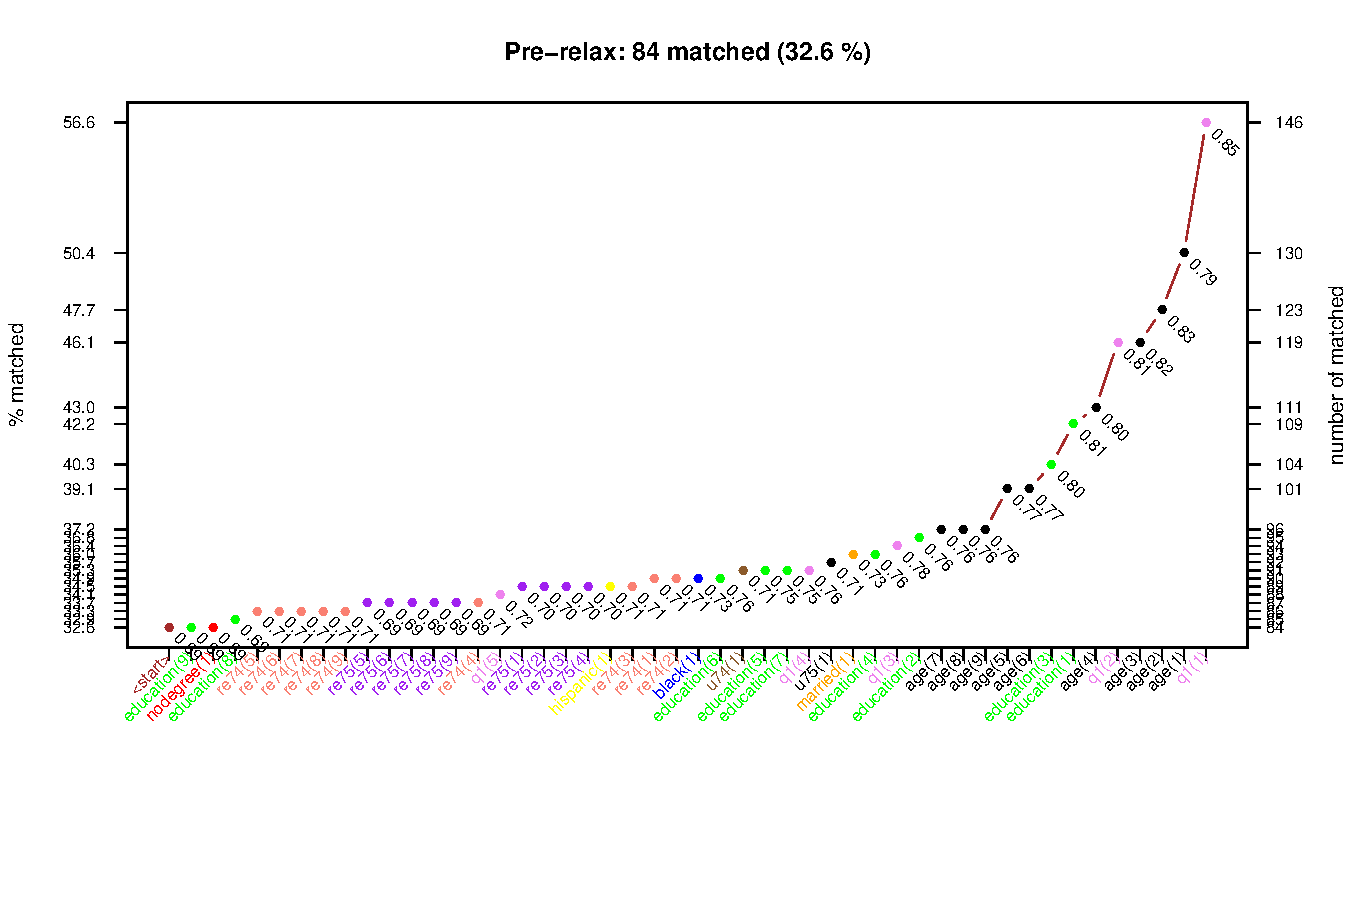
\includegraphics[width=1.1\textwidth, viewport=0 60 700 400,clip]{coarsen1} 
\end{center}
\caption{Example of the graphical output of $\tt relax.cem$.}
\label{fig:coarsen}
\end{figure}

After all possible coarsening relaxations are attempted, the function
returns a list of tables, one per group (i.e. treated and control).
Each row of the tables contain information about the number of treated
and control units matched, the value of the $\mathcal L_1$ measure,
and the type of relaxation made.  Each table is the sorted according
to the number of treated (or control) units matched.

The user may want to see the output of \code{tab\$G1} or
\code{tab\$G0} but these tables may be very long, and so we provide a
method \code{plot} to view these tables more conveniently.  The output
of \code{plot(tab)} is plotted in Figure \ref{fig:coarsen} from which
it is seen that the most difficult variables to match are \code{age}
and \code{education}.  On the $x$-axis of the plot the variable and
the number of equally sized bins used for the coarsening are used
(color-coded by variable).  On the $y$-axis on the right is the
absolute number of treated units matched, while the left side $y$-axis
reports the same number in percentages.  The numbers below the dots in
the graphs represent the $\mathcal L_1$ measure corresponding to that
matching solution.  This graph also gives a feeling of the MIB
behaviour of \code{cem}. When the tables produced by \code{relax.cem}
are too large, the \code{plot} function, allows for some reduction
like printing only the best matching solutions (in the terms of number
of treated units matched), removing duplicates (i.e. different
coarsenings may lead to the same matching solution), or printing only
solution where at least some percentage of treated units, have been
matched, or a combination of these. For more information refer to the
reference manual for the function \code{relax.plot} which can be
called directly instead of plot.

Here is one example of use of \code{plot} in which we specify that
only solutions with at least 60\% of the treated units are matched and
duplicated solutions are removed. The output can be seen in Figure
\ref{fig:coarsen2}

\begin{Schunk}
\begin{Sinput}
> plot(tab, group = "1", perc = 0.35, unique = TRUE)
\end{Sinput}
\end{Schunk}
\begin{figure}[Ht]
\begin{center}
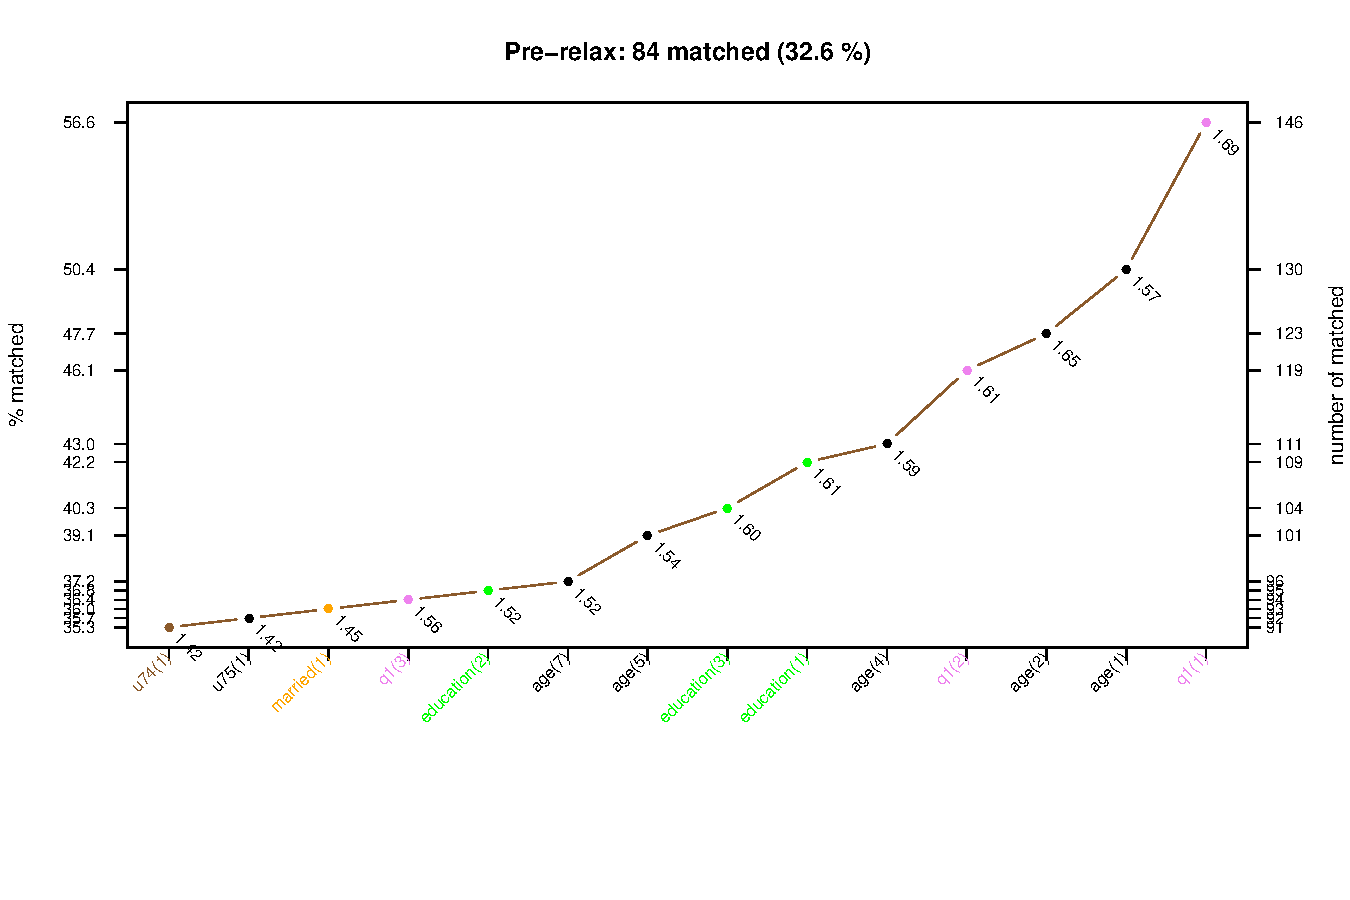
\includegraphics[width=1.1\textwidth,   viewport=0 60 700 400,clip]{coarsen2} 
\end{center}
\caption{Example of reduced graphical output of $\tt relax.cem$.}
\label{fig:coarsen2}
\end{figure}

\subsection{Restricting the Matching Solution to a $k$-to-$k$ Match}

By default, CEM uses maximal information, resulting in strata that may
include different numbers of treated and control units.  To compensate
for the differential strata sizes, \code{cem} also returns weights to
be used in subsequent analyses.  Although this is generally the best
option, a user with enough data may opt for a $k$-to-$k$ solution to
avoid the slight inconvenience of needing to use weights.

The function \code{k2k} accomplishes this by pruning observations from
a \code{cem} solution within each stratum until the solution contains
the same number of treated and control units in all strata.  Pruning
occurs within a stratum (for which observations are indistuinguishable
to cem proper) by using nearest neighbor selection using a distance
function specified by the user (including \code{euclidean},
\code{maximum}, \code{manhattan}, \code{canberra}, \code{binary}, or
\code{minkowski}). By default \code{method} is set to \code{NULL},
which means random matching inside \code{cem} strata, an option that
may reduce the chance for bias.  (For the Minkowski distance the power
can be specified via the argument \code{mpower}.  For more information
on \code{method != NULL}, refer to \code{dist} help page.)  

Here is an example of this approach.  First, by running \code{cem}:

\begin{Schunk}
\begin{Sinput}
> mat <- cem(treatment = "treated", data = Le, drop = "re78")
> mat
\end{Sinput}
\begin{Soutput}
           G0  G1
All       392 258
Matched    95  84
Unmatched 297 174


Multivariate Imbalance Measure: L1=0.605
Percentage of local common support: LCS=30.5%

Univariate Imbalance Measures:

           statistic   type        L1 min 25%   50%   75%    max
age        9.405e-02 (diff) 0.000e+00   0   0   1.0   0.0    0.0
education -2.222e-02 (diff) 2.222e-02   0   0   0.0   0.0    0.0
black      1.110e-16 (diff) 0.000e+00   0   0   0.0   0.0    0.0
married    0.000e+00 (diff) 0.000e+00   0   0   0.0   0.0    0.0
nodegree   0.000e+00 (diff) 0.000e+00   0   0   0.0   0.0    0.0
re74       1.496e+02 (diff) 0.000e+00   0   0   0.0 463.3  889.5
re75       1.588e+02 (diff) 0.000e+00   0   0 165.2 843.7 -640.9
hispanic   0.000e+00 (diff) 0.000e+00   0   0   0.0   0.0    0.0
u74        0.000e+00 (diff) 0.000e+00   0   0   0.0   0.0    0.0
u75        0.000e+00 (diff) 0.000e+00   0   0   1.0   0.0    0.0
q1         2.083e+00 (Chi2) 1.388e-17  NA  NA    NA    NA     NA
\end{Soutput}
\begin{Sinput}
> mat$k2k
\end{Sinput}
\begin{Soutput}
[1] FALSE
\end{Soutput}
\end{Schunk}
and now pruning to a $k$-to-$k$ solution, using the euclidean distance
within CEM strata:
\begin{Schunk}
\begin{Sinput}
> mat2 <- k2k(mat, Le, "euclidean", 1)
> mat2
\end{Sinput}
\begin{Soutput}
           G0  G1
All       392 258
Matched    70  70
Unmatched 322 188


Multivariate Imbalance Measure: L1=0.605
Percentage of local common support: LCS=30.5%

Univariate Imbalance Measures:

           statistic   type        L1 min 25%   50%   75%    max
age        9.405e-02 (diff) 0.000e+00   0   0   1.0   0.0    0.0
education -2.222e-02 (diff) 2.222e-02   0   0   0.0   0.0    0.0
black      1.110e-16 (diff) 0.000e+00   0   0   0.0   0.0    0.0
married    0.000e+00 (diff) 0.000e+00   0   0   0.0   0.0    0.0
nodegree   0.000e+00 (diff) 0.000e+00   0   0   0.0   0.0    0.0
re74       1.496e+02 (diff) 0.000e+00   0   0   0.0 463.3  889.5
re75       1.588e+02 (diff) 0.000e+00   0   0 165.2 843.7 -640.9
hispanic   0.000e+00 (diff) 0.000e+00   0   0   0.0   0.0    0.0
u74        0.000e+00 (diff) 0.000e+00   0   0   0.0   0.0    0.0
u75        0.000e+00 (diff) 0.000e+00   0   0   1.0   0.0    0.0
q1         2.083e+00 (Chi2) 1.388e-17  NA  NA    NA    NA     NA
\end{Soutput}
\begin{Sinput}
> mat2$k2k
\end{Sinput}
\begin{Soutput}
[1] TRUE
\end{Soutput}
\end{Schunk}
Alternatively, we can produce the same result in one step by adding
the \code{k2k=TRUE} option to the original \code{cem} call.

\subsection{Estimating the Causal Effect from CEM output}

Using the output from \code{cem}, we can estimate SATT via the
\code{att} function.  The simplest approach requires a weighted
difference in means (unless \code{k2k} was used, in which case no
weights are required).  For convenience, we compute this as a
regression of the outcome variable on a constant and the treatment variable,
\begin{Schunk}
\begin{Sinput}
> data(LL)
> mat <- cem(treatment = "treated", data = LL, drop = "re78")
> est <- att(mat, re78 ~ treated, data = LL)
> est
\end{Sinput}
\begin{Soutput}
           G0  G1
All       425 297
Matched   222 163
Unmatched 203 134

Linear regression model on CEM matched data:

SATT point estimate: 550.962564 (p.value=0.368242)
95% conf. interval: [-647.777701, 1749.702830]
\end{Soutput}
\end{Schunk}
where the SATT estimate is the coefficient on the \code{treated}
variable, in our case 550.96.  The function
\code{att} allows for \proglang{R}'s standard \code{formula} interface and, by
default, uses a linear model to estimate the att using the weights 
produced by \code{cem}.  

If exact matching (i.e., without coarsening) was chosen this procedure
is appropriate as is.  In other situations, with some coarsening, some
imbalance remains in the matched data.  The remaining imbalance is
strictly bounded by the level of coarsening, which can be seen by any
remaining variation within the coarsened bins.  Thus, a reasonable
approach in this common situation is to attempt to adjust for the
remaining imbalance via a statistical model.  (Modeling assumptions
for models applied to the matched data are much less consequential
than they would otherwise be because CEM is known to strictly bound
the level of model dependence.)  To apply a statistical model to
control for the remaining imbalance, we use the \code{formula}
interface in \code{att}.  For example:

\begin{Schunk}
\begin{Sinput}
> est2 <- att(mat, re78 ~ treated + re74, data = LL)
> est2
\end{Sinput}
\begin{Soutput}
           G0  G1
All       425 297
Matched   222 163
Unmatched 203 134

Linear regression model on CEM matched data:

SATT point estimate: 553.113736 (p.value=0.362760)
95% conf. interval: [-636.606542, 1742.834014]
\end{Soutput}
\end{Schunk}

The user can also specify the option \code{model} which accepts one of the following string arguments
\begin{itemize}
\item \code{linear} or \code{lm} (the default) for linear model, when the treatment effect is supposed to be homogeneous
\begin{Schunk}
\begin{Sinput}
> att(mat, re78 ~ treated + re74, data = LL, model = "linear")
\end{Sinput}
\begin{Soutput}
           G0  G1
All       425 297
Matched   222 163
Unmatched 203 134

Linear regression model on CEM matched data:

SATT point estimate: 553.113736 (p.value=0.362760)
95% conf. interval: [-636.606542, 1742.834014]
\end{Soutput}
\end{Schunk}
\item \code{linear-RE} or \code{lme} for linear model with random effects in cem strata, for non-homogeneous treatment effect
\begin{Schunk}
\begin{Sinput}
> att(mat, re78 ~ treated + re74, data = LL, model = "linear-RE")
\end{Sinput}
\begin{Soutput}
           G0  G1
All       425 297
Matched   222 163
Unmatched 203 134

Linear random effect model on CEM matched data:

SATT point estimate: 552.448961 (p.value=0.000000)
95% conf. interval: [364.067068, 740.830853]
\end{Soutput}
\end{Schunk}
\item \code{logistic} or \code{logit} for dichotomous response variable\footnote{We do not provide an example here, model the syntax is the same for the other models.},  for homogeneous treatment effect. 
\item \code{forest} or \code{rf} for random forest  model, also for non-homogeneous treatment effect. It accepts continuous, dichotomous or counting outcomes.
\begin{Schunk}
\begin{Sinput}
> att(mat, re78 ~ treated + re74, data = LL, model = "forest")
\end{Sinput}
\begin{Soutput}
           G0  G1
All       425 297
Matched   222 163
Unmatched 203 134

Random forest model on CEM matched data:

SATT point estimate: 535.568997 (p.value=0.551682)
95% conf. interval: [-1227.908618, 2299.046613]
\end{Soutput}
\end{Schunk}
\end{itemize}
All the above models run on the CEM matched subsamples, so the quantity of interest may change in case of non-homogeneous treatment effect.
The option \code{extrapolate}, if set \code{TRUE}, extrapolates each of the above models also to the set of treated units not matched. In this case the quantity of interest is kept fixed but the estimation is more model dependent.
\begin{Schunk}
\begin{Sinput}
> att(mat, re78 ~ treated + re74, data = LL, model = "linear", 
+     extra = TRUE)
\end{Sinput}
\begin{Soutput}
           G0  G1
All       425 297
Matched   222 163
Unmatched 203 134

Linear regression model with extrapolation:

SATT point estimate: 674.337762 (p.value=0.347286)
95% conf. interval: [-236.091964, 1584.767489]
\end{Soutput}
\begin{Sinput}
> att(mat, re78 ~ treated + re74, data = LL, model = "linear-RE", 
+     extra = TRUE)
\end{Sinput}
\begin{Soutput}
           G0  G1
All       425 297
Matched   222 163
Unmatched 203 134

Linear random effect model with extrapolation:

SATT point estimate: 902.087484 (p.value=0.000000)
95% conf. interval: [816.567245, 987.607724]
\end{Soutput}
\begin{Sinput}
> att(mat, re78 ~ treated + re74, data = LL, model = "rf", extra = TRUE)
\end{Sinput}
\begin{Soutput}
           G0  G1
All       425 297
Matched   222 163
Unmatched 203 134

Random forest model with extrapolation:

SATT point estimate: 32.951232 (p.value=0.960063)
95% conf. interval: [-1256.786364, 1322.688829]
\end{Soutput}
\end{Schunk}
As Figure \ref{fig:teff} shows, it is also possible to plot the results of the SATT estimation as follows
\begin{Schunk}
\begin{Sinput}
> est3 <- att(mat, re78 ~ treated + re74, data = LL)
> est3
\end{Sinput}
\begin{Soutput}
           G0  G1
All       425 297
Matched   222 163
Unmatched 203 134

Linear regression model on CEM matched data:

SATT point estimate: 553.113736 (p.value=0.362760)
95% conf. interval: [-636.606542, 1742.834014]
\end{Soutput}
\begin{Sinput}
> plot(est3, mat, LL, vars = c("education", "age", "re74", "re75"))
\end{Sinput}
\end{Schunk}
\begin{figure}[Ht]
\begin{center}
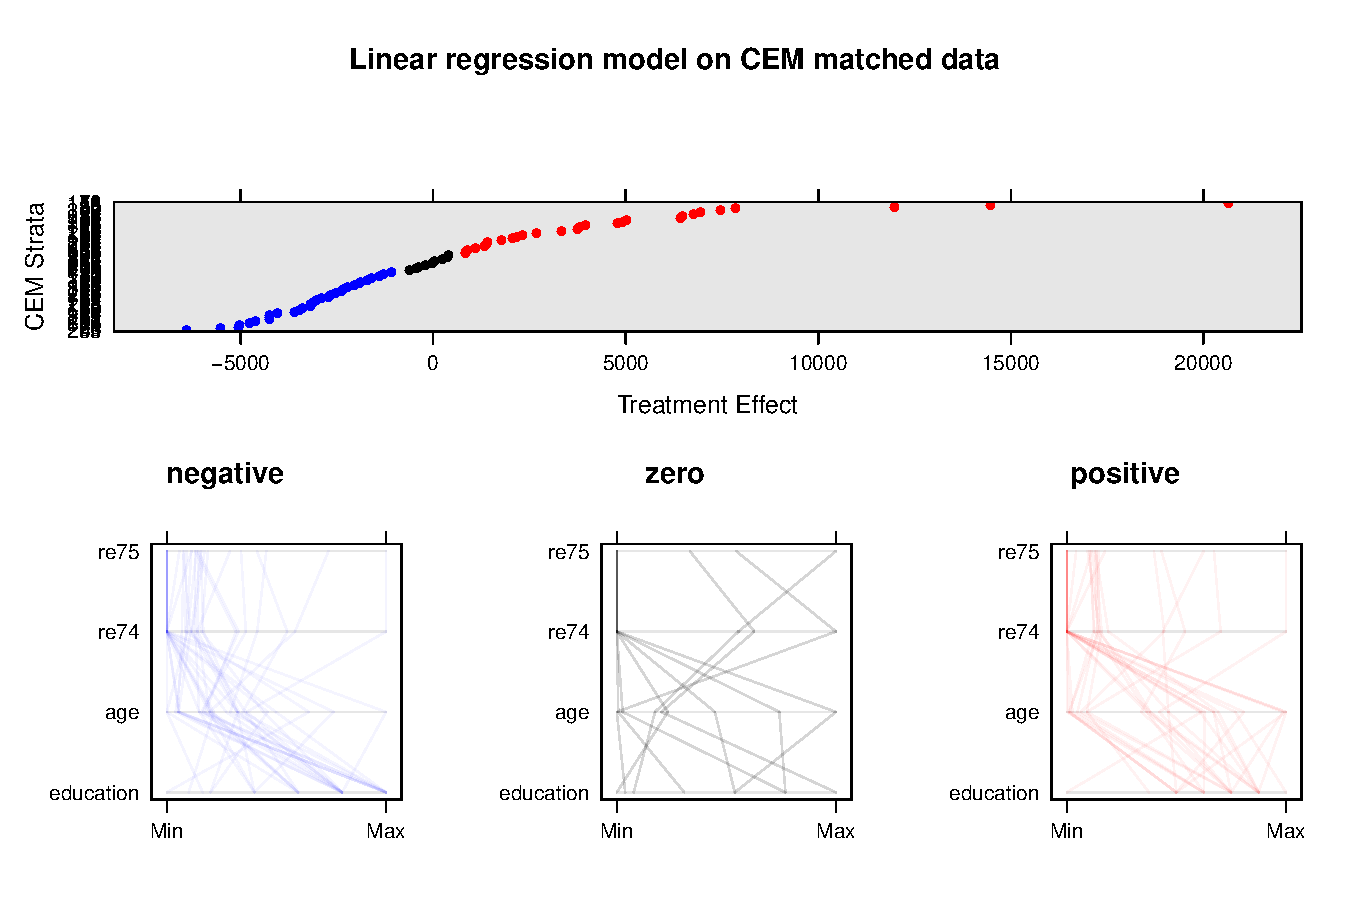
\includegraphics[width=0.9\textwidth]{teff} 
\end{center}
\caption{Example of a plot of the output of $\tt att$.  The top panel
  gives observation-level causal effect estimates sorted in numerical
  order and colored in ranges -- negative (in blue), not significantly
  different from zero (black), or positive (red).  For each range of
  effects, the bottom panel gives parallel plots; each line in a
  parallel plot represents the (covariate) characteristics of a single
  observation.}
\label{fig:teff}
\end{figure}
For more
information, see the reference manual entry for \code{att}.




\subsection{Matching and Missing Data}\label{s:mv}

Almost all previous methods of matching assume the absence of any
missing values.  In contrast, CEM offers two valid approaches to
dealing with missing values (item nonresponse).  In the first, where
we treat missing values as one of the values of the variables, is
appropriate when ``\code{NA}'' is a valid value that is not really
missing (such as when ``no opinion'' really means no opinion); see
Section \ref{s:mvdirect}.  The other is a special procedure to allow
for multiply imputed data in CEM, as described in Section
\ref{s:mvmi}.

\subsubsection{Matching on Missingness}\label{s:mvdirect}

In the next example, we use our original \code{LeLonde} data with
missing values and we compare the result with \code{Le} from which we
dropped the \code{NA} values.  For comparability, we use the same
cutpoints we used in Section \ref{sec:cem} on the \code{Le} data. The
cutpoints are contained in \code{mat\$breaks}

\begin{Schunk}
\begin{Sinput}
> mat3 <- cem("treated", LeLonde, drop = "re78", cutpoints = mat$breaks, 
+     grouping = list(q1 = q1.grp))
\end{Sinput}
\begin{Soutput}
Missing values exist in the data!
\end{Soutput}
\begin{Sinput}
> mat3
\end{Sinput}
\begin{Soutput}
           G0  G1
All       425 297
Matched   134 101
Unmatched 291 196


Multivariate Imbalance Measure: L1=0.723
Percentage of local common support: LCS=27.5%

Univariate Imbalance Measures:

          statistic   type        L1 min 25% 50% 75%    max
age       1.893e-01 (diff) 0.000e+00   0   0   0   0    0.0
education 0.000e+00 (diff) 0.000e+00   0   0   0   0    0.0
black     0.000e+00 (diff) 5.551e-17   0   0   0   0    0.0
married   0.000e+00 (diff) 0.000e+00   0   0   0   0    0.0
nodegree  1.110e-16 (diff) 0.000e+00   0   0   0   0    0.0
re74      4.563e+01 (diff) 0.000e+00   0   0   0 543  889.5
re75      8.120e+01 (diff) 0.000e+00   0   0   0 816 -640.9
hispanic  0.000e+00 (diff) 0.000e+00   0   0   0   0    0.0
u74       0.000e+00 (diff) 2.776e-17   0   0   0   0    0.0
u75       0.000e+00 (diff) 0.000e+00   0   0   0   0    0.0
q1        3.822e+00 (Chi2) 7.084e-02  NA  NA  NA  NA     NA
\end{Soutput}
\end{Schunk}
and we compare the above with the solution obtained by dropping the observations with missing data
\begin{Schunk}
\begin{Sinput}
> mat4 <- cem("treated", Le, drop = "re78", cutpoints = mat$breaks, 
+     grouping = list(q1 = q1.grp))
> mat4
\end{Sinput}
\begin{Soutput}
           G0  G1
All       392 258
Matched   132 100
Unmatched 260 158


Multivariate Imbalance Measure: L1=0.734
Percentage of local common support: LCS=27.5%

Univariate Imbalance Measures:

          statistic   type        L1 min 25% 50% 75%    max
age       1.919e-01 (diff) 0.000e+00   0   0   0   0    0.0
education 1.776e-15 (diff) 0.000e+00   0   0   0   0    0.0
black     0.000e+00 (diff) 3.469e-18   0   0   0   0    0.0
married   0.000e+00 (diff) 0.000e+00   0   0   0   0    0.0
nodegree  1.110e-16 (diff) 0.000e+00   0   0   0   0    0.0
re74      4.583e+01 (diff) 0.000e+00   0   0   0 543  889.5
re75      8.287e+01 (diff) 0.000e+00   0   0   0 816 -640.9
hispanic  0.000e+00 (diff) 1.735e-18   0   0   0   0    0.0
u74       0.000e+00 (diff) 0.000e+00   0   0   0   0    0.0
u75       0.000e+00 (diff) 2.776e-17   0   0   0   0    0.0
q1        3.698e+00 (Chi2) 7.279e-02  NA  NA  NA  NA     NA
\end{Soutput}
\end{Schunk}

and, as expected, the two solutions differ somewhat. The gain (in
terms of number of matched units) decreases as the number of
covariates increases.

\subsubsection{Matching Multiply Imputed Data}\label{s:mvmi}

Consider a data set to be matched, some of which is missing. One
approach to analyzing data with missing values is \emph{multiple
imputation}, which involves creating $m$ (usually about $m=5$) data
sets, each of which is the same as the original except that the
missing values have been imputed in each.  Uncertainty in the values
of the missing cells is represented by variation in the imputations
across the different imputed data sets \citep{KinHonJos01}.

As an example we take the original \code{LeLonde} data with missing values
\begin{Schunk}
\begin{Sinput}
> summary(LeLonde)
\end{Sinput}
\begin{Soutput}
    treated           age         education        black        married     
 Min.   :0.000   Min.   :17.0   Min.   : 3.0   Min.   :0.0   Min.   :0.000  
 1st Qu.:0.000   1st Qu.:19.0   1st Qu.: 9.0   1st Qu.:1.0   1st Qu.:0.000  
 Median :0.000   Median :23.0   Median :10.0   Median :1.0   Median :0.000  
 Mean   :0.411   Mean   :24.5   Mean   :10.3   Mean   :0.8   Mean   :0.163  
 3rd Qu.:1.000   3rd Qu.:27.0   3rd Qu.:11.0   3rd Qu.:1.0   3rd Qu.:0.000  
 Max.   :1.000   Max.   :55.0   Max.   :16.0   Max.   :1.0   Max.   :1.000  
                 NA's   : 8.0   NA's   : 8.0   NA's   :1.0   NA's   :9.000  
    nodegree          re74            re75            re78      
 Min.   :0.000   Min.   :    0   Min.   :    0   Min.   :    0  
 1st Qu.:1.000   1st Qu.:    0   1st Qu.:    0   1st Qu.:    0  
 Median :1.000   Median :  824   Median :  941   Median : 4033  
 Mean   :0.778   Mean   : 3662   Mean   : 3051   Mean   : 5486  
 3rd Qu.:1.000   3rd Qu.: 5237   3rd Qu.: 3993   3rd Qu.: 8813  
 Max.   :1.000   Max.   :39571   Max.   :37432   Max.   :60308  
 NA's   :5.000   NA's   :    8   NA's   :    4   NA's   :    7  
    hispanic           u74             u75                        q1     
 Min.   : 0.000   Min.   :0.000   Min.   :0.000   agree            :111  
 1st Qu.: 0.000   1st Qu.:0.000   1st Qu.:0.000   disagree         :121  
 Median : 0.000   Median :0.000   Median :0.000   neutral          :129  
 Mean   : 0.104   Mean   :0.453   Mean   :0.402   no opinion       :117  
 3rd Qu.: 0.000   3rd Qu.:1.000   3rd Qu.:1.000   strongly agree   :121  
 Max.   : 1.000   Max.   :1.000   Max.   :1.000   strongly disagree:118  
 NA's   :11.000   NA's   :3.000   NA's   :3.000   NA's             :  5  
\end{Soutput}
\end{Schunk}
Now we use \code{Amelia} package \citep{HonKinBLa06} to create
multiply imputed data sets:
\begin{Schunk}
\begin{Sinput}
> require(Amelia)
\end{Sinput}
\begin{Soutput}
## 
## Amelia II: Multiple Imputation
## (Version 1.2-0, built: 2009-04-02)
## Copyright (C) 2005-2009 James Honaker, Gary King and Matthew Blackwell
## Refer to http://gking.harvard.edu/amelia/ for more information
##
\end{Soutput}
\begin{Sinput}
> set.seed(123)
> imputed <- amelia(LeLonde, noms = c("black", "hispanic", "treated", 
+     "married", "nodegree", "u74", "u75", "q1"))
\end{Sinput}
\begin{Soutput}
-- Imputation 1 --

 1  2  3 

-- Imputation 2 --

 1  2  3  4 

-- Imputation 3 --

 1  2  3 

-- Imputation 4 --

 1  2  3  4 

-- Imputation 5 --

 1  2  3 
\end{Soutput}
\begin{Sinput}
> imputed <- imputed$imputations[1:5]
\end{Sinput}
\end{Schunk}

Now \code{imputed} contains a list of 5 multiply imputed versions of
\code{LeLonde}.  We pass this list to the \code{cem} function in the argument
\code{datalist} and \code{cem} produces a set of multiply imputed
solutions, as usual with the original uncoarsened values of the
variables, but now assigning each multiply imputed observation to the
strata where it falls most frequently.  The output of \code{cem} is a
list of \code{cem.match} solutions (named \code{match1},
\code{match2},\dots, \code{match5}).  (Be sure to also name the
original data frame in option \code{data} or \code{cem} will merely
run the basic algorithm five separate times on each of the input data
sets, a procedure that can be useful for batch processing of data to
be matched, but is not recommended for multiply imputed data sets
since the strata will not be the same across the data sets.)  For
example:
\begin{Schunk}
\begin{Sinput}
> mat2 <- cem("treated", datalist = imputed, drop = "re78", data = LeLonde, 
+     grouping = list(q1 = q1.grp))
> mat2
\end{Sinput}
\begin{Soutput}
           G0  G1
All       425 297
Matched   132  98
Unmatched 293 199


Multivariate Imbalance Measure: L1=0.703
Percentage of local common support: LCS=28.3%

Univariate Imbalance Measures:

          statistic   type       L1    min 25% 50%    75%    max
age       -0.141910 (diff) 0.000000    0.0  -1   0    0.0    0.0
education -0.003269 (diff) 0.017007    0.0   0   0    0.0    0.0
black      0.000000 (diff) 0.000000    0.0   0   0    0.0    0.0
married   -0.003061 (diff) 0.005102    0.0   0   0    0.0    0.0
nodegree  -0.002041 (diff) 0.000000    0.0   0   0    0.0    0.0
re74      99.066521 (diff) 0.000000 -250.6   0   0  252.3 -197.1
re75      44.619415 (diff) 0.000000    0.0   0   0 -128.5  640.9
hispanic   0.001531 (diff) 0.007653    0.0   0   0    0.0    0.0
u74        0.004082 (diff) 0.000000    0.0   0   0    0.0    0.0
u75        0.000000 (diff) 0.000000    0.0   0   0    0.0    0.0
q1         2.141127 (Chi2) 0.061905     NA  NA  NA     NA     NA
\end{Soutput}
\end{Schunk}

Now we estimate SATT via the usual multiple imputation combining
formulas (averaging the point estimates and within and between
variances, as usual; see \citep{KinHonJos01}).  The function
\code{att} implements these procedures:
\begin{Schunk}
\begin{Sinput}
> out <- att(mat2, re78 ~ treated, data = imputed)
> out
\end{Sinput}
\begin{Soutput}
Linear regression model on CEM matched data:

SATT point estimate: 1177.182780 (p.value=0.123993)
95% conf. interval: [-322.747427, 2677.112987]
\end{Soutput}
\end{Schunk}

\subsection{Creating paired samples}
In same cases, it is useful to apply CEM so some data to create paired matched samples.
Given an output of \code{cem}, the function \code{pair} produces two sets of indexes corresponding to pair matched units.
\begin{Schunk}
\begin{Sinput}
> data(LL)
> mat <- cem(data = LL, drop = "re78")
> psample <- pair(mat, data = LL)
\end{Sinput}
\begin{Soutput}
Total number of units paired in CEM strata: 352
Total number of units matched: 722
\end{Soutput}
\end{Schunk}
each pair of observation has a different strata number
\begin{Schunk}
\begin{Sinput}
> table(psample$paired)[1:50]
\end{Sinput}
\begin{Soutput}
 1  2  3  4  5  6  7  8  9 10 11 12 13 14 15 16 17 18 19 20 21 22 23 24 25 26 
 2  2  2  2  2  2  2  2  2  2  2  2  2  2  2  2  2  2  2  2  2  2  2  2  2  2 
27 28 29 30 31 32 33 34 35 36 37 38 39 40 41 42 43 44 45 46 47 48 49 50 
 2  2  2  2  2  2  2  2  2  2  2  2  2  2  2  2  2  2  2  2  2  2  2  2 
\end{Soutput}
\end{Schunk}
not all observations can be matched in cem strata
\begin{Schunk}
\begin{Sinput}
> psample$paired[1:50]
\end{Sinput}
\begin{Soutput}
15993 15994 15995 15996 15997 15998 15999 16000 16001 16002 16003 16004 16005 
   NA    NA    NA    NA    NA    NA    NA    NA    NA    NA    NA    NA    NA 
16006 16007 16008 16009 16010 16011 16012 16013 16014 16015 16016 16017 16018 
   NA    NA    NA    NA    NA    NA    NA    NA    NA    NA    NA    NA    NA 
16019 16020 16021 16022 16023 16024 16025 16026 16027 16028 16029 16030 16031 
   NA    NA    NA    NA    NA     1    NA    NA    NA     1    NA    NA    NA 
16032 16033 16034 16035 16036 16037 16038 16039 16040 16041 16042 
   NA    NA    NA    NA    NA    NA    NA    NA    NA    NA    NA 
\end{Soutput}
\end{Schunk}
the remaining observations are then matched and the final list of all paired units is
contained in the filed \code{full.paired}
\begin{Schunk}
\begin{Sinput}
> table(psample$full.paired)[1:50]
\end{Sinput}
\begin{Soutput}
 1  2  3  4  5  6  7  8  9 10 11 12 13 14 15 16 17 18 19 20 21 22 23 24 25 26 
 2  2  2  2  2  2  2  2  2  2  2  2  2  2  2  2  2  2  2  2  2  2  2  2  2  2 
27 28 29 30 31 32 33 34 35 36 37 38 39 40 41 42 43 44 45 46 47 48 49 50 
 2  2  2  2  2  2  2  2  2  2  2  2  2  2  2  2  2  2  2  2  2  2  2  2 
\end{Soutput}
\begin{Sinput}
> psample$full.paired[1:10]
\end{Sinput}
\begin{Soutput}
15993 15994 15995 15996 15997 15998 15999 16000 16001 16002 
  265   268   240   189   196   195   267   177   227   232 
\end{Soutput}
\end{Schunk}
When the data contain an even number of units, all units can be
paired; if they cannot be paired, the function indicates which units are
left without a mate.
\begin{Schunk}
\begin{Sinput}
> mat1 <- cem(data = LL[-1, ], drop = "re78")
> psample <- pair(mat1, data = LL[-1, ])
\end{Sinput}
\begin{Soutput}
Total number of units paired in CEM strata: 352
Total number of units matched: 720
Unit corresponding to row `15994', not paired
\end{Soutput}
\begin{Sinput}
> table(psample$full.paired)[1:50]
\end{Sinput}
\begin{Soutput}
 1  2  3  4  5  6  7  8  9 10 11 12 13 14 15 16 17 18 19 20 21 22 23 24 25 26 
 2  2  2  2  2  2  2  2  2  2  2  2  2  2  2  2  2  2  2  2  2  2  2  2  2  2 
27 28 29 30 31 32 33 34 35 36 37 38 39 40 41 42 43 44 45 46 47 48 49 50 
 2  2  2  2  2  2  2  2  2  2  2  2  2  2  2  2  2  2  2  2  2  2  2  2 
\end{Soutput}
\end{Schunk}



\bibliography{cem}
\end{document}
